\documentclass[a4paper, twoside]{article}

%% Language and font encodings
\usepackage[english]{babel}
\usepackage[utf8x]{inputenc}
\usepackage[T1]{fontenc}

%% Sets page size and margins
\usepackage[a4paper,top=3cm,bottom=2cm,left=3cm,right=3cm,marginparwidth=1.75cm]{geometry}

%% Useful packages
\usepackage{amsmath}
\usepackage{graphicx}
\usepackage[colorinlistoftodos]{todonotes}
\usepackage[colorlinks=true, allcolors=blue]{hyperref}
\usepackage{url}
\usepackage{multicol}
\usepackage{graphicx}
\usepackage{caption}
\usepackage{subcaption}
\setcounter{secnumdepth}{3}
\usepackage[margin=1cm]{caption}


\title{}
\author{Abra\~{a}o Pacheco Dos Santos Peres Mota}

\begin{document}
	
	\begin{center}
	\Large{467H - Principles of Decentralized Ledgers
		
		Smart Contracts Coursework} 
	
	\Large{Abra\~{a}o Pacheco Dos Santos Peres Mota - }
	\large{\textbf{CID:} 00941232}
	\end{center}

\section{Introduction}

I have opted to write a smart contract implementing a game of rock paper scissors. Due to their existence in the blockchain, as well as no enforced guarantees as to when a player must take their turn, this otherwise simple game becomes more complex due to security concerns. I have imported a string utility library from \url{https://github.com/Arachnid/solidity-stringutils} for easier string manipulation. 

\section{Game Architecture}

The game has 4 distinct stages, each of which are separated by user driven actions. These comprise:

\begin{enumerate}
	\item \textbf{Game registration} - This is the first step taken in the game. Before the game proceeds, both players must have registered their interest in partaking in the game. This stage allocates the callers \texttt{address} to be set to either Player 1 or Player 2, if either of these are available at the moment. If they are not available, the contract caller is not considered a valid player, so any attempts at calling any subsequent steps will fail. Registration comes at a price - the players must provide a minimum entry price to enter the game (like a bet), so that the winner may receive a price and monetary rewards can be duly distributed to the miners of the transactions involved in the game. This contract only allows for 1 game at any given time, so any existing game must finish before any other game can commence.
	
	\item \textbf{Move commitment} - Due to security concerns of using the blockchain, the game follows a \textit{Commit-Reveal} approach. In this stage of the game, the player commits to a specific move. They do this by submitting a signature to the game,  comprised of the \texttt{keccak256} hash of the string made up by \texttt{move + salt}, where the \texttt{move} is one of \texttt{"rock"}, \texttt{"paper"} or \texttt{"scissors"}. The \texttt{salt} is a random string of the players choice used to hash their move. This salt should be kept secret until the reveal stage of the game.
	
	\item \textbf{Move reveal} - At this stage, the player reveals their move of choice to the contract. They do so by submitting their \texttt{move} and \texttt{salt} in plaintext when calling the \texttt{revealMove} function. After this submission, the contract checks whether this is the valid move that the player has committed to previously; if the signature that was submitted in the commit phase does not match the \texttt{keccak256} hash of the \texttt{move} and the \texttt{hash} that were passed in at this stage, then the player is seen to be attempting to cheat - they have committed to a signed move but when revealing they attempt to provide a different move. 
	
	\item \textbf{Checking for end of game} - This function checks for the sufficient conditions to finish the game in question. This can happen in 1 of 2 ways - either both players have revealed their moves within a reasonable threshold of one another, or one player has waited a sufficiently long time after revealing (in this contract, the waiting threshold is set to 5 minutes). If one of these conditions has been met, then the game is considered to be over, and the winner is decided. If any player has been considered to be cheating at any point in the game, they will not receive any of the winnings (unless both players have cheated, in which case the game is considered a draw, and the winnings are split equally between the two). 
\end{enumerate}

\begin{figure}
	\centering
	\begin{subfigure}{.5\textwidth}
		\centering
		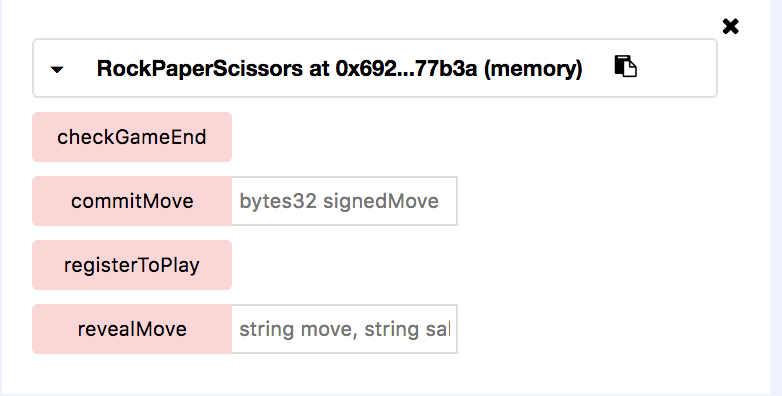
\includegraphics[width=\linewidth]{screens/solidityAPI.png}
		\captionsetup{width=.95\linewidth}
	
		\caption[width=0.8\linewidth]{The interaction API to the contract as seen in \textit{Remix}}
		\label{fig:sub1}
	\end{subfigure}%
	\begin{subfigure}{.5\textwidth}
		\centering
		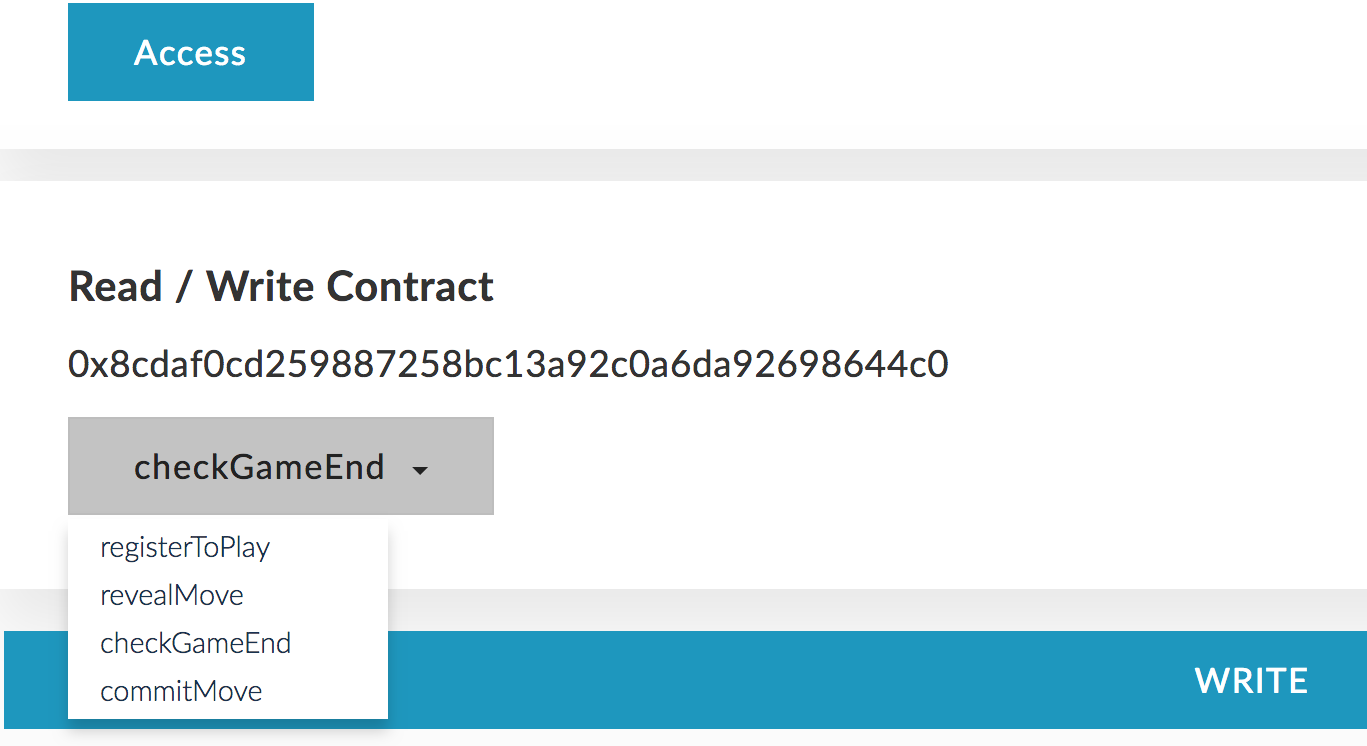
\includegraphics[width=\linewidth]{screens/ether3}
		      \captionsetup{width=.95\linewidth}
		
		\caption[width=0.8\linewidth]{Interacting with the contract using \textit{myEtherWallet}}
		\label{fig:sub2}
	\end{subfigure}
	\label{fig:test}
\end{figure}



\begin{figure}[!h]
	\centering
	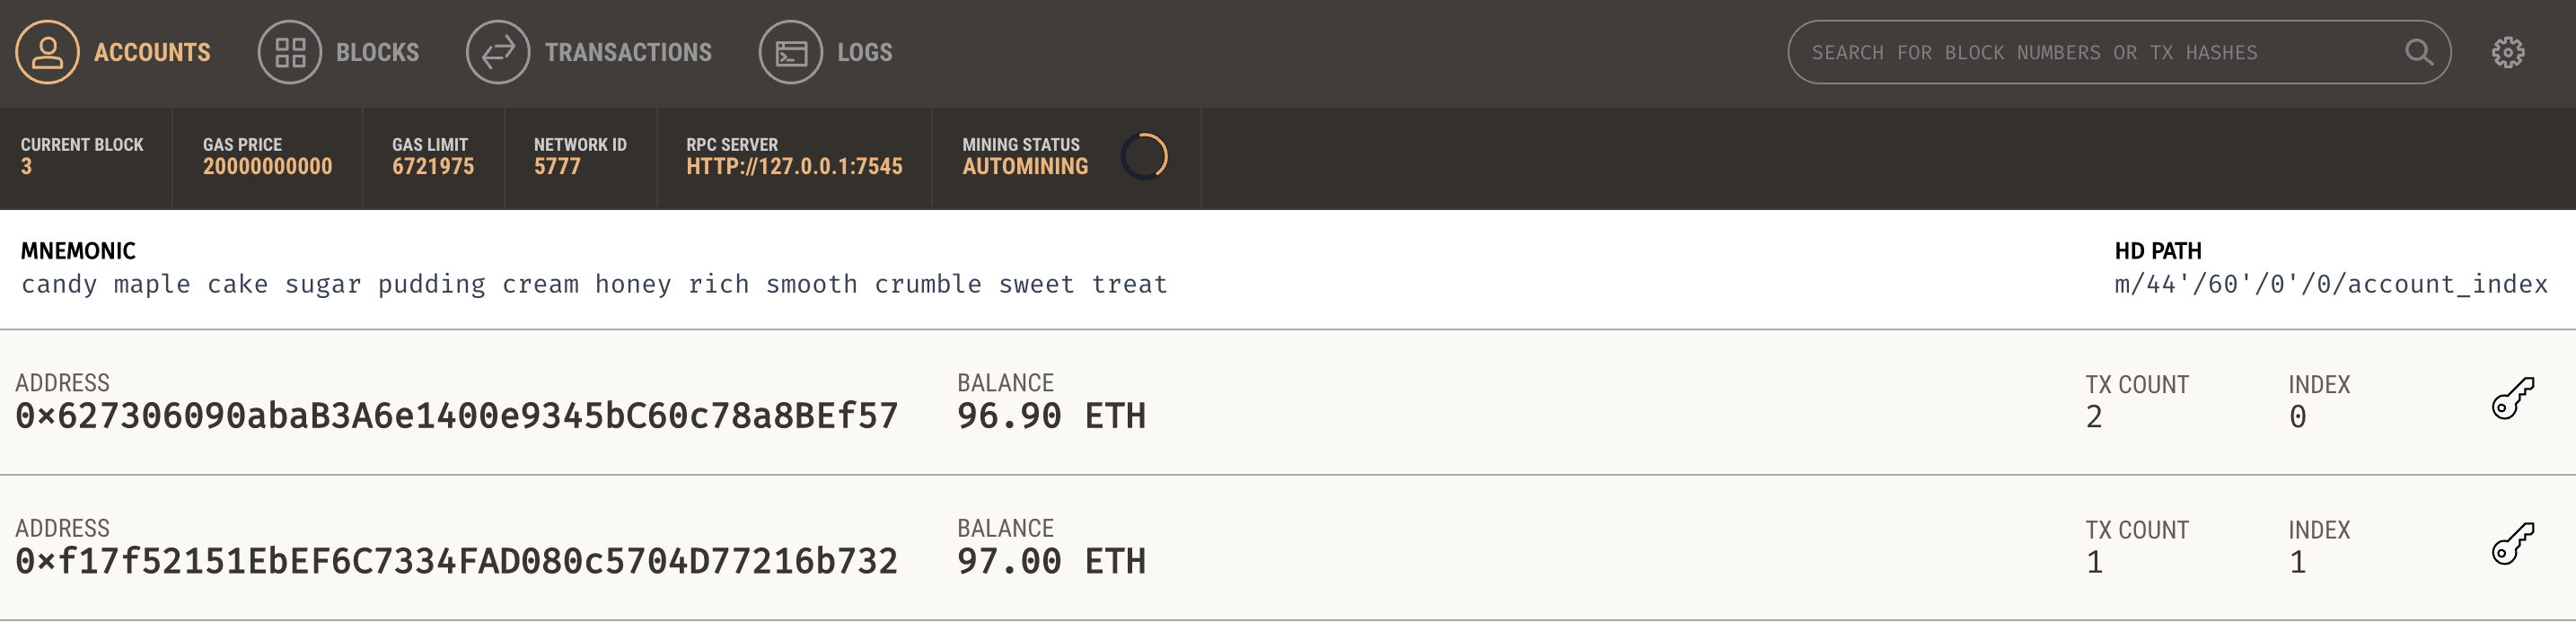
\includegraphics[width=\textwidth]{screens/postRegistration.png}	
	\caption{An ongoing game after player registration. Note the first address also created the contract, hence the discrepancy between the balance of the 2 accounts.}
\end{figure}
\begin{figure}[!h]
	\centering
	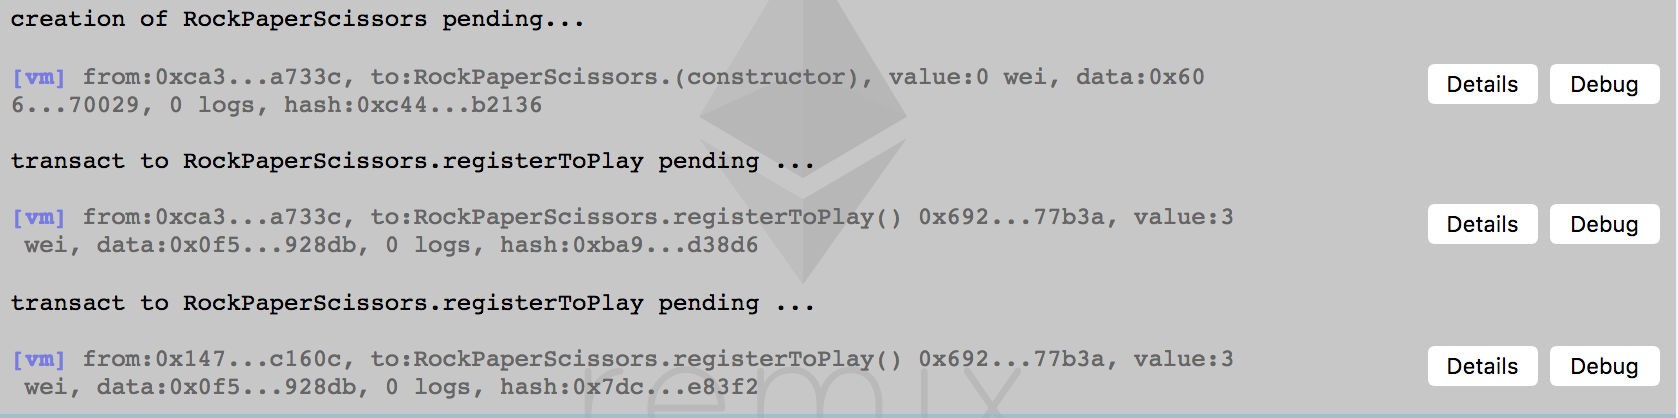
\includegraphics[width=\textwidth]{screens/initialTransactions.png}	
	\caption{Transactions being triggered in Remix - here we see the creation of a game and 2 players registering to play.}
\end{figure}
\begin{figure}[!h]
	\centering
	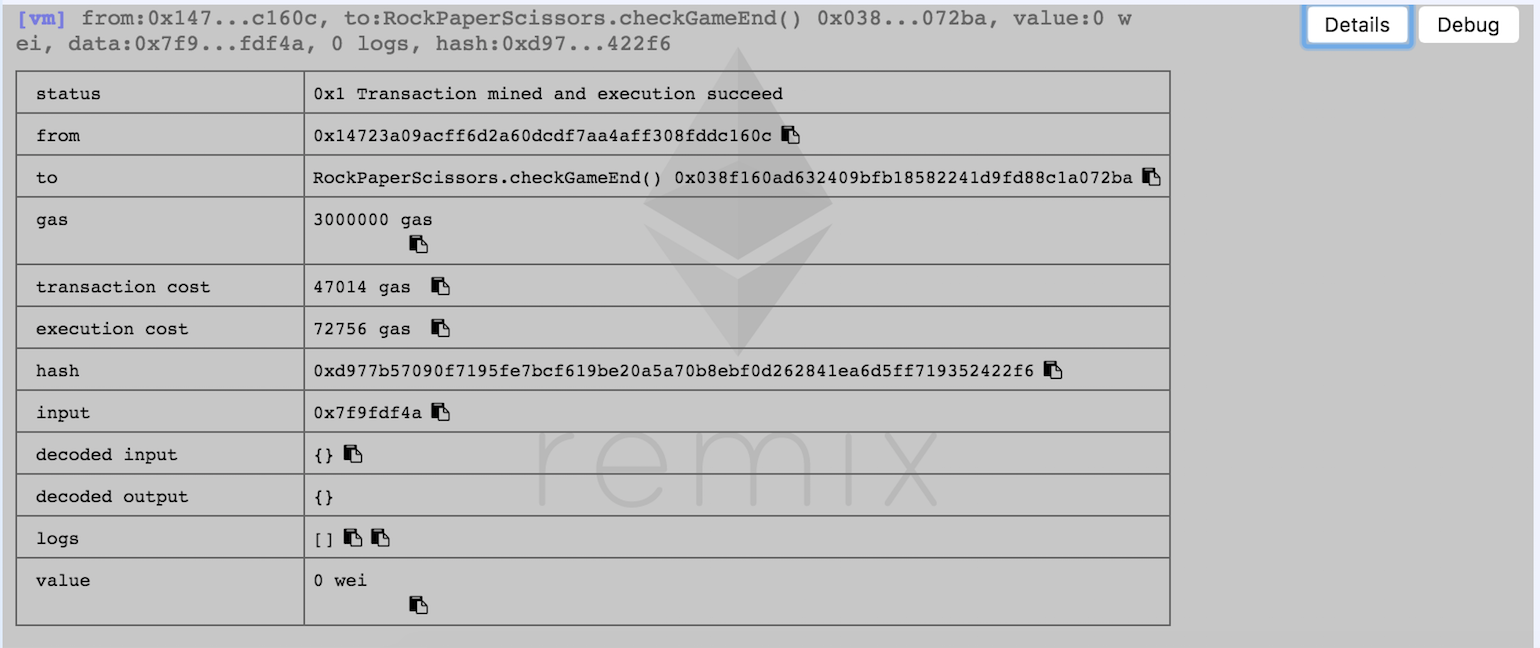
\includegraphics[width=\textwidth]{screens/gameEnd.png}	
	\caption{A final game transaction in Remix - the game finishes successfully in this case.}
\end{figure}
\begin{figure}[!h]
	\centering
	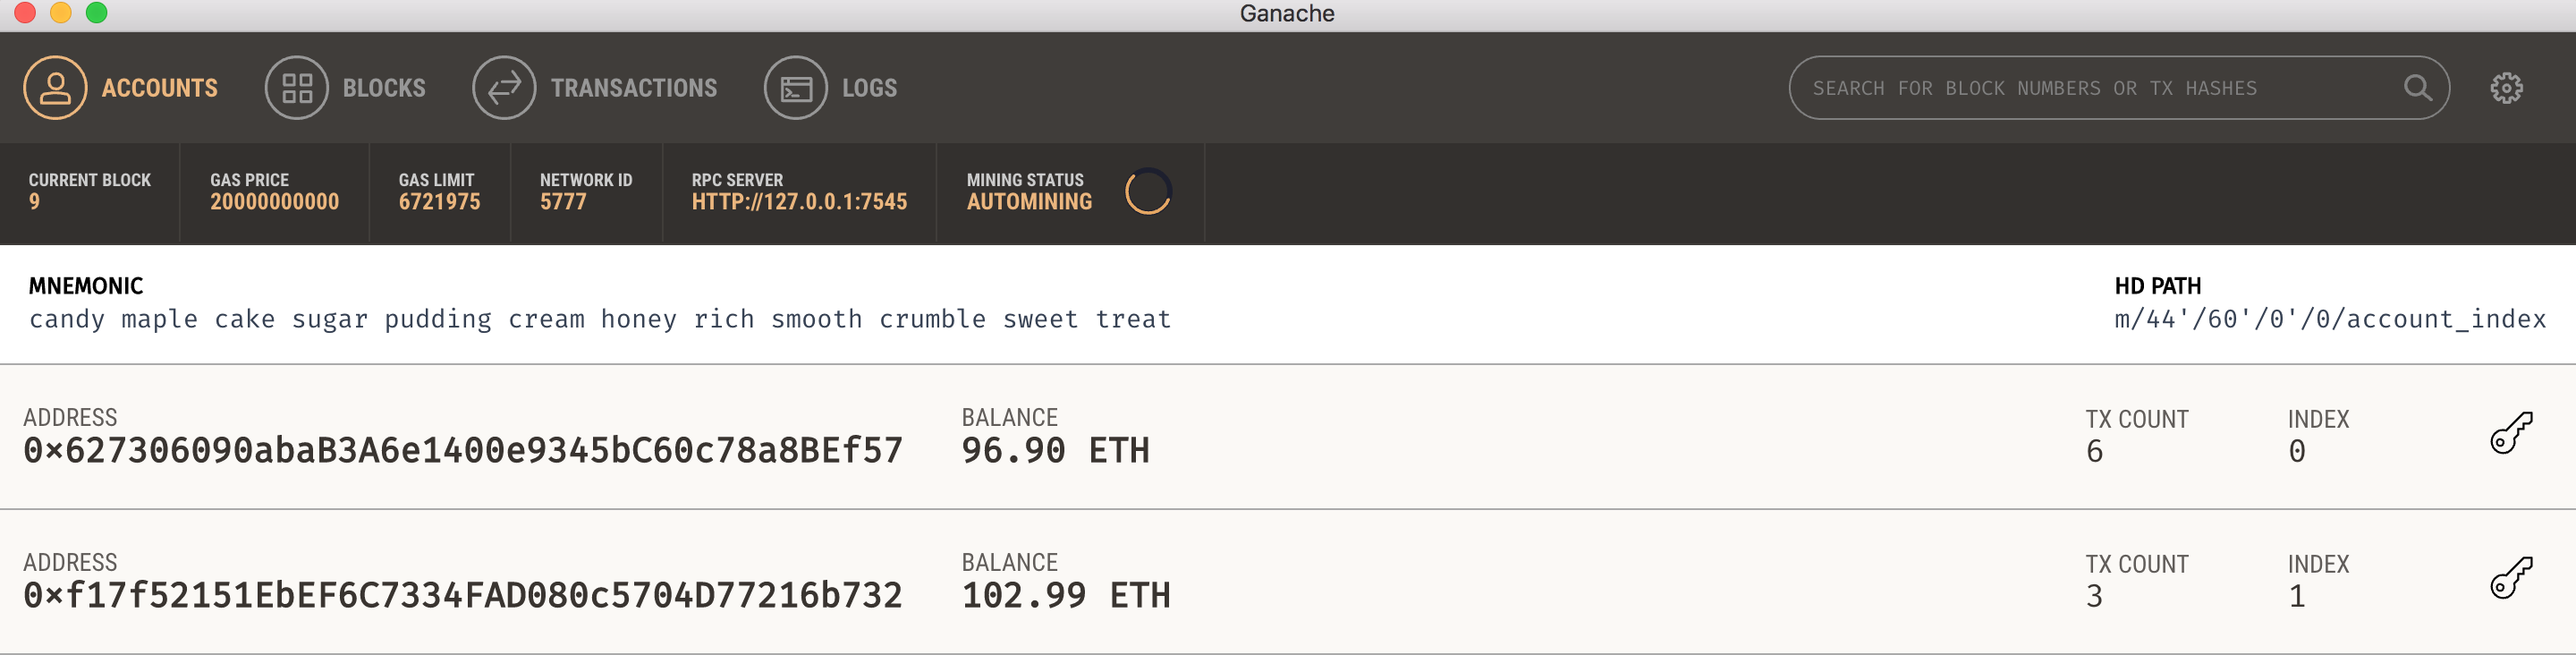
\includegraphics[width=\textwidth]{screens/matchEnd.png}	
	\caption{At the end of a game with an equal bet of 3 \textit{ETH}, the second player wins the bet (discrepancies in values go towards contract creation and transaction fees).}
\end{figure}
\section{Threat Modelling}

As it stands, the game must assume the worst of both players to be able to execute in a fair way that rewards players appropriately. There are a number of different ways in which a player could attempt to cheat the system.

\begin{itemize}
	\item \textbf{Read opponents move or change your own move} - This is the biggest security concern of implementing this game in the blockchain. All the information on the blockchain is stored in full sight of every user, and the smart contract writer cannot guarantee that both players play their move at the same time - as soon as a user submits their move, the transaction containing this information becomes public. The opponent could inspect this transaction and thus change their move accordingly to win the game everytime. Due to this, a \textit{Commit-Reveal} approach must be used to safeguard both parties. This works by ensuring that both players commit to a move before they reveal their move to the blockchain. The commit phase is done by submitting a signature that fits a pre-defined format (in our case, it is the output of running \texttt{keccak256(move + salt)} in \textit{Solidity}). Because the \textit{salt} is a player chosen attribute, the user can submit the signature without letting others know what his move is. The \textit{salt} can then be used in the reveal phase to verify the signature. The \textit{Commit-Reveal} approach relies on the fact that reversing the produced \texttt{keccak256} signature (finding the inputs required to generate the signature given) is computationally infeasible for the game players. If this could be reversed, then the move could be obtained as soon as the signature is uploaded to the blockchain, rendering this approach useless in securing the game against cheaters.
	
	\item \textbf{Denial of Service} - Given we are using the \textit{Commit-Reveal} approach, a malicious player could still attempt to ruin the game. Suppose that both players have committed to a a move, and then Player 1 reveals his move. This has made his move public to Player 2, and may reveal to Player 2 that he will lose the game (e.g. Player 1 has picked \textit{"rock"} and Player 2 is \textit{"scissors"}). Player 2 may then choose to deny the end of the game from happening by choosing to never reveal his move. In order to decentivise this deviant behaviour, the game sets a maximum waiting threshold of 5 minutes after the first move reveal by any player for the other player to also reveal their move. If the second revealer still hasn't revealed his move after this time threshold has elapsed when the \texttt{checkGameEnd} function is called, then this player is declared to be a cheater.
	
	\item \textbf{Tamper with existing games} - Given that the contract is in the public domain, any caller may attempt to call the public functions provided by the contract. Since the contract only supports one game at a time, it will only allow the registered players to call game state changing functions. The entry point to the contract finite state machine (the \texttt{registerToPlay} function), will have no effect when called if there are no more spaces in the game, meaning unregistered players will have no effect on an ongoing game.
\end{itemize}

\subsection{Strategy Rewards}

Given that a player may still choose to attempt to cheat, it is important to calculate what their average expected winnings are - if a cheating strategy has the same or higher expected winnings as an honest strategy, there is no rational incentive for playing honestly. \\

Assuming the current game is able to detect all forms of cheating, the expected return \textit{E\textsubscript{1}} for a cheating strategy will be negative. This covers different cases:

\begin{enumerate}
	\item \textbf{Cheater vs Honest} - The game detects cheating in this case, and transfers the contract balance to the Honest player.
	\item \textbf{Cheater vs Cheater} - The game detects both players are cheating, and splits the contract balance accordingly. However, due to transaction costs the players incurr in playing the game, in the case of this "draw", the players cannot make an expected return that is greater than 0.
\end{enumerate} 

On the other hand, we analyse the expected return \textit{E\textsubscript{2}} for an honest player:

\begin{enumerate}
	\item \textbf{Honest vs Cheater} - As before, the game detects the other player is cheating, and transfers the contract balance to the Honest player. The Honest player thus makes a profit on the game, winning the entry fee that the Cheater required to register for the game.
	\item \textbf{Honest vs Honest} - In this case, the expected return is the same as that of a normal Rock Paper Scissors game, whereby assuming both players make a choice at random, they have an equal chance of doubling their entry fee, drawing or losing their initial bet.
\end{enumerate}

From this low-level analysis, we can see that the worst-case scenario for \textit{E\textsubscript{1}} and \textit{E\textsubscript{2}} is the same (the player loses their entry bet), whereas the best-case scenario for \textit{E\textsubscript{2}} doubles the player's initial investment, when the best outcome from \textit{E\textsubscript{1}} is a "draw" against another cheater, resulting in an outcome that adds up to slightly less than the initial investment. Thus it becomes clear that the honest strategy \textit{E\textsubscript{2}} is the more financially rewarding of the two.

\section{Extensions and Further Concerns}

In order to improve the implementation of this contract, there are further concerns and improvements that could be dealt with. These include:

\begin{itemize}
	
	\item \textbf{Paying the contract maker} - At the moment, the contract has no inherent mechanism to incentivise the creation of the contract itself. This transaction costs a small amount of ether, but whoever calls this functionality does not get rewarded for doing so. In a better case scenario, the owner of the address that called the contract constructor should be rewarded with a percentage of the winner's winnings. 
	
	\item \textbf{Allow for concurrent games} - As the contract stands, it only allows for one game at a time per contract. It is feasible however to support multiple concurrent games, by implementing a mapping of game id's to a new object (\texttt{Game} perhaps) which stores all the state for any given game. In this way, players would be registered into either a game with one awaiting player or a new game if there are no players queueing to play. 
	
	\item \textbf{Enforcing equal entry bets} - In order for the game to be fair, players should be entering an equal bet into the game. Although the game enforces that players make a minimum bet to enter, there is no constraint on whether a player bets more than this. A misinformed player might bet significantly more than his opponent, for no quantifiable advantage over their smaller and less risky bet. 
	
	\item \textbf{Enforcing minimum salt length} - The salt used by a player should be long enough to make it computationally infeasible to reverse a function in the given game time. In a bad approach, a player may use the letter \texttt{"b"} as their salt. In this case, it is feasible to imagine an alphabetically brute-force approach to cracking the produced \texttt{keccak256} of the \texttt{move + salt}. Assuming the player is honest and they play a valid move, there are only 3 potential strings to check - \texttt{keccak256("rockb")}, \texttt{keccak256("paperb")} and \texttt{keccak256("scissorsb")}. In this case, the opponent could figure out the hashed move and salt and adjust his playing strategy accordingly. Enforcing minimum salt lengths (8 characters minimum for example), may be a good approach. However, this would be an approach that should be handled by a frontend to the contract - the salt is only revealed after a player commits to a move, so it may become frustrating to play the game if a player commits to a signature using a salt they only realise is invalid after their commitment.
	
	\item \textbf{Web interface} - A web interface would allows players to easily interact with the contract. In this frontend some constraints mentioned above (such as equal entry bets and minimum salt length) would be easier to approach and constrain using Javascript. A concern to this would be to ensure that the implementations of the hashing algorithm \texttt{keccak256} used in the frontend are the same as those used in \textit{Solidity}.
	
\end{itemize}


\end{document}